\section{Suggestions to Improve the Existing System}

\subsection{System Perspective}

\subsection{External Interfaces}

\vfill
\begin{figure}[H]
  \centering
  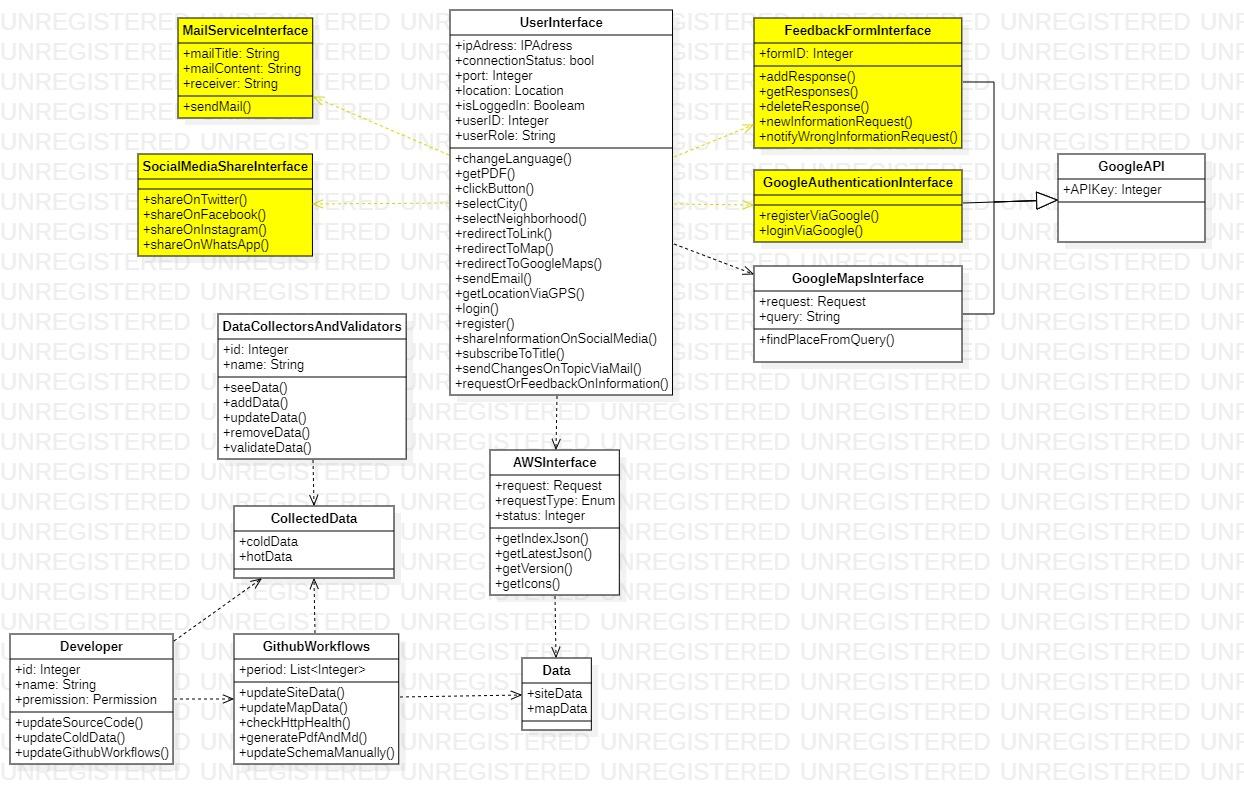
\includegraphics[width=\linewidth]{img/external-interfaces-s4.jpg}
  \caption{Suggested New External Interfaces}
\end{figure}
\vfill
\newpage

\subsection{Functions}

\subsection{Usability Requirements}

\subsection{Performance Requirements}

\subsection{Logical Database Requirements}

\afetbilgi does currently have a relational database. To make minor difference in the source code, the object structure in the Section 3.5 is preserved. Additionally, users, roles and mail subscription data are added into database. \texttt{Users} relation provides information related to the login system. \texttt{Roles} relation provides information related to the registered role. \texttt{Mail Subscription} relation provides the information related to topics that users subcribed.

\begin{figure}[H]
  \centering
  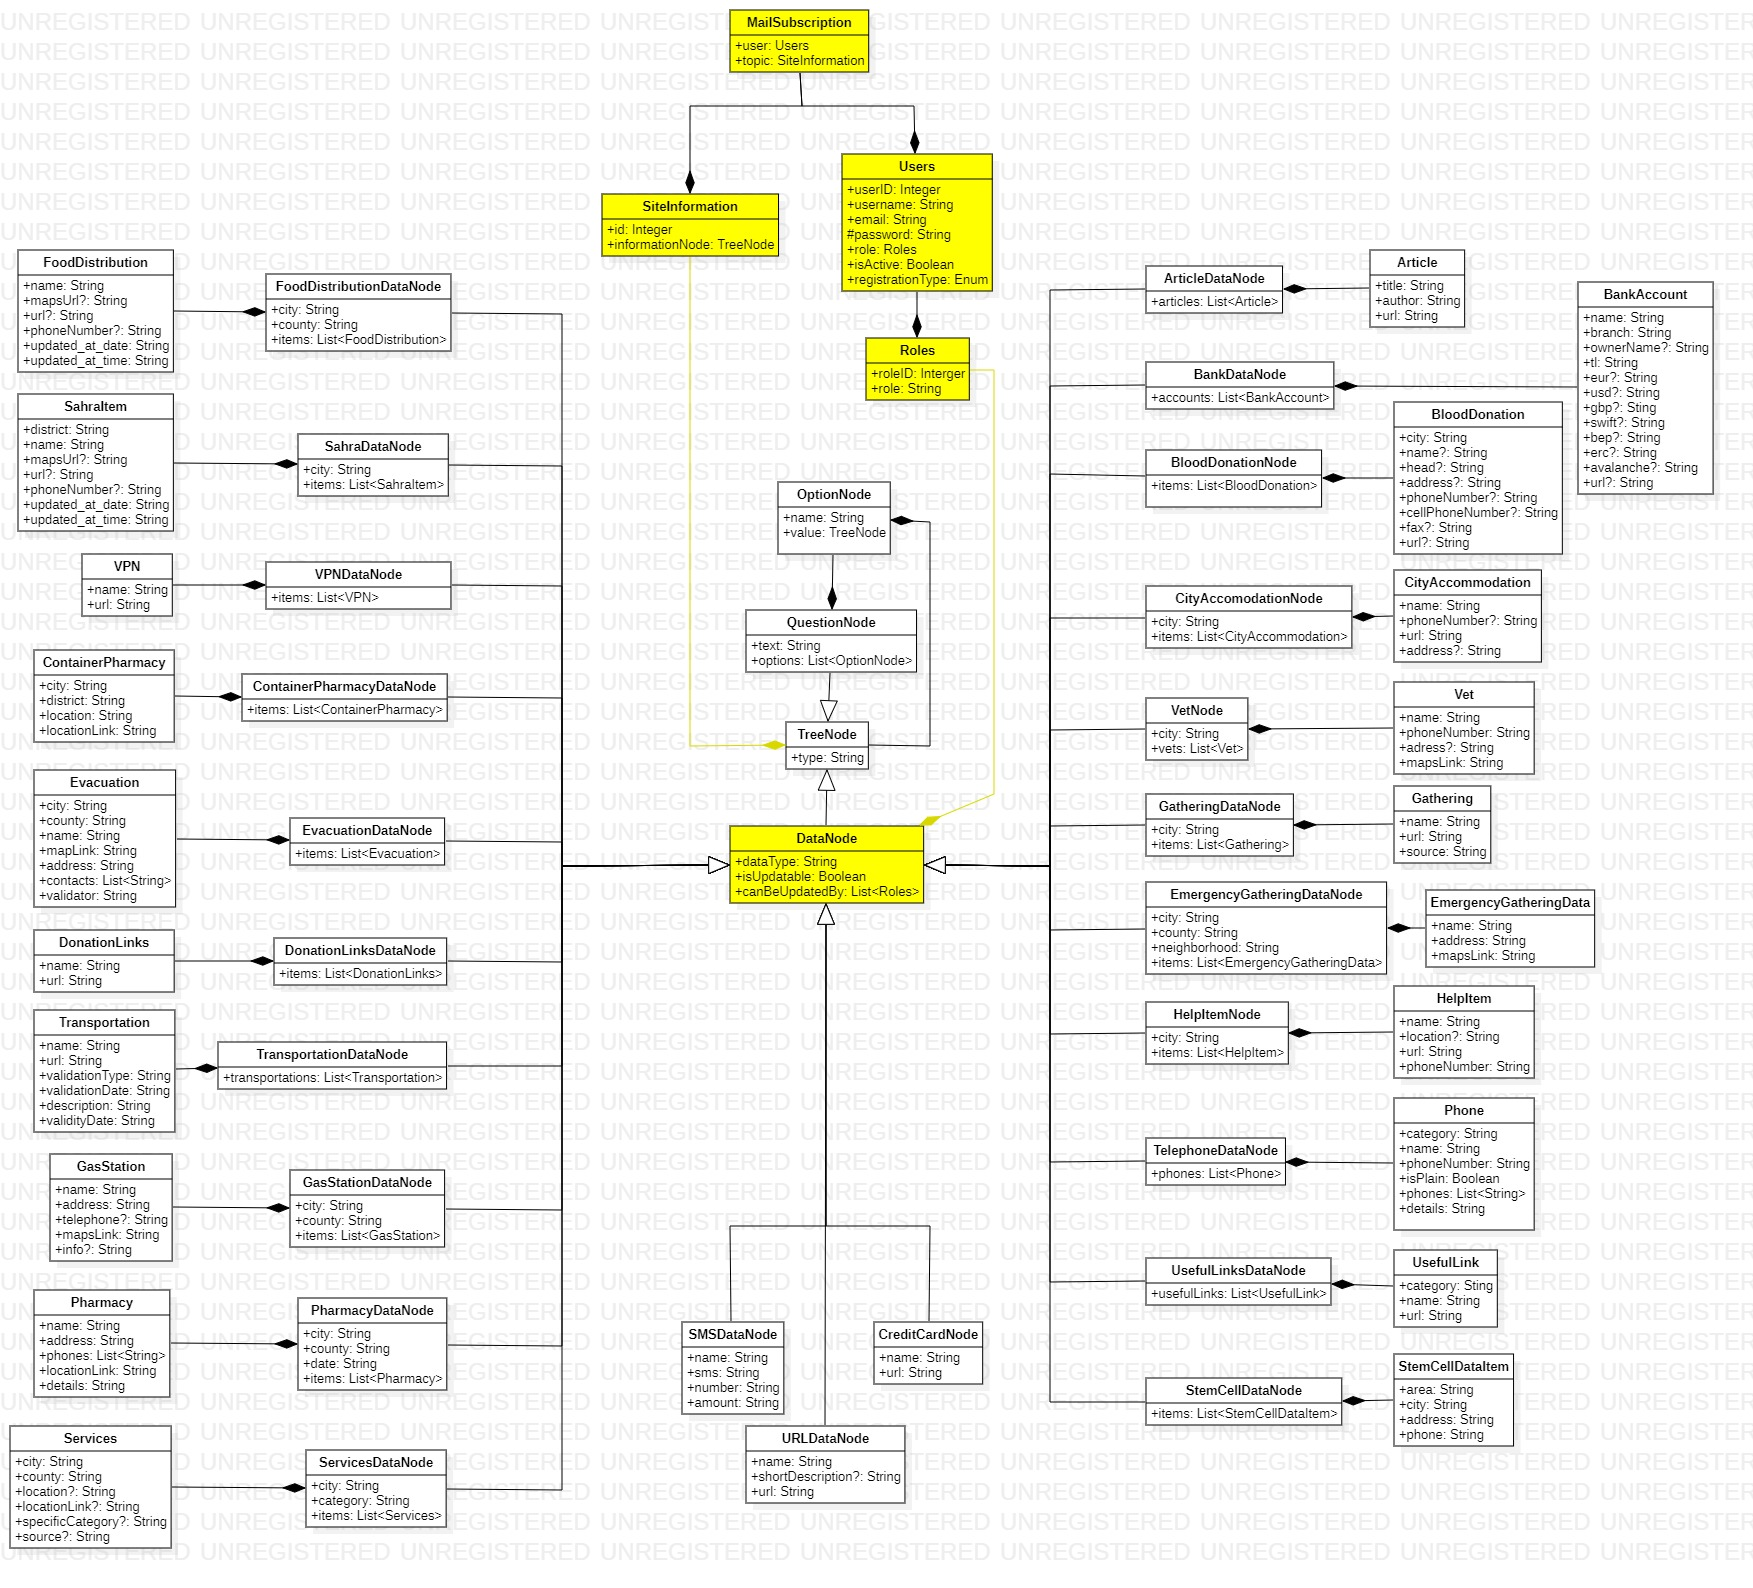
\includegraphics[width=\linewidth]{img/database-s4.jpg}
  \caption{Suggested New Relational Database}
\end{figure}

\subsection{Design Constraints}

\subsection{System Attributes}

\subsection{Supporting Information}
